\documentclass[10pt]{article}
\usepackage[paperwidth=10.6in,paperheight=4.7in,margin=0.15in]{geometry}
\usepackage{amsmath,amssymb,bm}
\usepackage{tikz}
\usetikzlibrary{arrows.meta,positioning,calc,fit,backgrounds}
\pagestyle{empty}
\definecolor{inputgray}{RGB}{76,84,92}
\definecolor{predblue}{RGB}{42,104,145}
\definecolor{controlred}{RGB}{181,74,58}
\definecolor{controlorange}{RGB}{196,116,42}
\definecolor{fitpurple}{RGB}{102,75,145}
\begin{document}
\centering
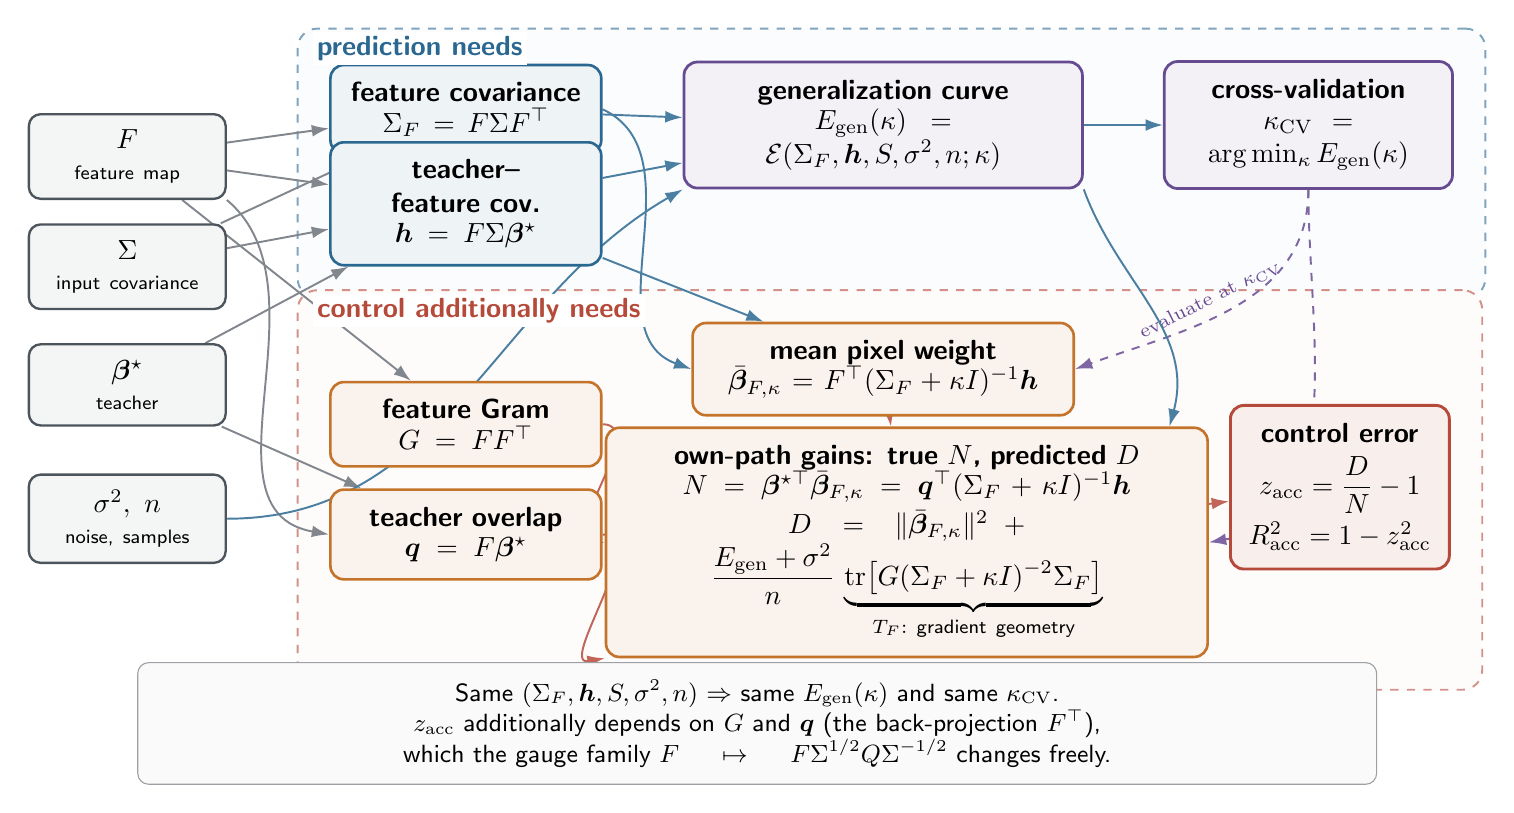
\begin{tikzpicture}[
  x=1cm,y=1cm,font=\sffamily,>=Latex,
  dep/.style={-{Latex[length=2.2mm,width=1.5mm]},draw=inputgray!70,line width=0.7pt},
  pdep/.style={dep,draw=predblue!85},
  cdep/.style={dep,draw=controlred!85},
  kdep/.style={dep,draw=fitpurple!85,dashed},
  input/.style={draw=inputgray,line width=0.85pt,rounded corners=1.5mm,fill=inputgray!6,
                text width=2.1cm,minimum height=0.9cm,align=center,inner sep=2mm},
  pstat/.style={draw=predblue,line width=0.95pt,rounded corners=1.7mm,fill=predblue!8,
                text width=3.0cm,minimum height=1.0cm,align=center,inner sep=2.2mm},
  cstat/.style={draw=controlorange,line width=0.95pt,rounded corners=1.7mm,fill=controlorange!9,
                text width=3.0cm,minimum height=1.0cm,align=center,inner sep=2.2mm},
  fitbox/.style={draw=fitpurple,line width=1.0pt,rounded corners=1.7mm,fill=fitpurple!8,
              text width=4.6cm,minimum height=1.0cm,align=center,inner sep=2.3mm},
  cout/.style={draw=controlred,line width=1.05pt,rounded corners=1.7mm,fill=controlred!9,
               align=center,inner sep=2.3mm},
  group/.style={draw,line width=0.7pt,dashed,rounded corners=2.5mm,inner sep=4mm}
]
% ---------- inputs
\node[input] (F)     at (0,2.9)  {$F$\\[-1pt]\scriptsize feature map};
\node[input] (Sigma) at (0,1.5)  {$\Sigma$\\[-1pt]\scriptsize input covariance};
\node[input] (beta)  at (0,0.0)  {$\bm\beta^\star$\\[-1pt]\scriptsize teacher};
\node[input] (noise) at (0,-1.7) {$\sigma^2,\ n$\\[-1pt]\scriptsize noise, samples};
% ---------- prediction summaries
\node[pstat] (SF) at (4.3,3.5) {\textbf{feature covariance}\\[-1pt]$\Sigma_F=F\Sigma F^\top$};
\node[pstat] (h)  at (4.3,2.3) {\textbf{teacher--feature cov.}\\[-1pt]$\bm h=F\Sigma\bm\beta^\star$};
% ---------- control summaries
\node[cstat] (G) at (4.3,-0.5) {\textbf{feature Gram}\\[-1pt]$G=FF^\top$};
\node[cstat] (q) at (4.3,-1.9) {\textbf{teacher overlap}\\[-1pt]$\bm q=F\bm\beta^\star$};
% ---------- prediction outputs
\node[fitbox] (Egen) at (9.6,3.3)
  {\textbf{generalization curve}\\[-1pt]$E_{\rm gen}(\kappa)=\mathcal E(\Sigma_F,\bm h,S,\sigma^2,n;\kappa)$};
\node[fitbox,text width=3.2cm] (kcv) at (15.0,3.3)
  {\textbf{cross-validation}\\[-1pt]$\kappa_{\rm CV}=\arg\min_\kappa E_{\rm gen}(\kappa)$};
% ---------- control outputs
\node[cstat,text width=4.4cm] (bt) at (9.6,0.2)
  {\textbf{mean pixel weight}\\[-1pt]$\bar{\bm\beta}_{F,\kappa}=F^\top(\Sigma_F+\kappa I)^{-1}\bm h$};
\node[cstat,text width=7.2cm] (ND) at (9.9,-2.0)
  {\textbf{own-path gains: true $N$, predicted $D$}\\[-1pt]
   $N=\bm\beta^{\star\top}\bar{\bm\beta}_{F,\kappa}=\bm q^\top(\Sigma_F+\kappa I)^{-1}\bm h$\\[2pt]
   $D=\|\bar{\bm\beta}_{F,\kappa}\|^2+\dfrac{E_{\rm gen}+\sigma^2}{n}\,\underbrace{\operatorname{tr}\!\big[G(\Sigma_F+\kappa I)^{-2}\Sigma_F\big]}_{T_F:\ \text{gradient geometry}}$};
\node[cout] (z) at (15.4,-1.3)
  {\textbf{control error}\\[4pt]$z_{\rm acc}=\dfrac{D}{N}-1$\\[2pt]$R^2_{\rm acc}=1-z_{\rm acc}^2$};
% ---------- groups and arrows
\begin{scope}[on background layer]
  \node[group,draw=predblue!60,fill=predblue!2,fit=(SF)(h)(Egen)(kcv)] (pg) {};
  \node[group,draw=controlred!60,fill=controlred!2,fit=(G)(q)(bt)(ND)(z)] (cg) {};
  \draw[dep] (F) -- (SF);   \draw[dep] (Sigma) -- (SF);
  \draw[dep] (F) -- (h);    \draw[dep] (Sigma) -- (h);   \draw[dep] (beta) -- (h);
  \draw[dep] (F) -- (G);
  \draw[dep] (F.south east) to[out=-40,in=170] (q.west); \draw[dep] (beta) -- (q);
  \draw[pdep] (SF) -- (Egen);  \draw[pdep] (h) -- (Egen);
  \draw[pdep] (noise.east) to[out=0,in=-150] (Egen.south west);
  \draw[pdep] (Egen) -- (kcv);
  \draw[kdep] (kcv.south) to[out=-90,in=20] node[pos=0.55,above,sloped,font=\scriptsize,text=fitpurple] {evaluate at $\kappa_{\rm CV}$} (bt.east);
  \draw[kdep] (kcv.south) to[out=-90,in=10] (ND.east);
  \draw[pdep] (SF.east) to[out=-25,in=160] (bt.west);  \draw[pdep] (h) -- (bt);
  \draw[cdep] (G.east) to[out=0,in=180] (ND.west);
  \draw[cdep] (q.east) to[out=0,in=190] (ND.south west);
  \draw[cdep] (bt) -- (ND);
  \draw[pdep] (Egen.south east) to[out=-70,in=75] ([xshift=-5mm]ND.north east);
  \draw[cdep] (ND) -- (z);
\end{scope}
\node[font=\bfseries\sffamily,text=predblue,fill=white,inner sep=1.5pt,anchor=north west] at ([xshift=2mm,yshift=-0.5mm]pg.north west) {prediction needs};
\node[font=\bfseries\sffamily,text=controlred,fill=white,inner sep=1.5pt,anchor=north west] at ([xshift=2mm,yshift=-0.5mm]cg.north west) {control additionally needs};
\node[draw=inputgray!55,fill=black!2,rounded corners=1.4mm,text width=15.5cm,align=center,inner ysep=2.2mm,font=\small\sffamily]
  at (8.0,-4.3)
  {Same $(\Sigma_F,\bm h,S,\sigma^2,n)$ $\Rightarrow$ same $E_{\rm gen}(\kappa)$ and same $\kappa_{\rm CV}$.\\
   $z_{\rm acc}$ additionally depends on $G$ and $\bm q$ (the back-projection $F^\top$), which the gauge family $F\mapsto F\Sigma^{1/2}Q\Sigma^{-1/2}$ changes freely.};
\end{tikzpicture}
\end{document}
